%%%%%%%%%%%%%%%%%%%%%%%%%%%%%%%%%%%%%%%%%%%%%%%%%%%%%%%%%%%%%%%%%%%%%%%%%%%%%%%%
\documentclass[twocolumn]{revtex4}

%%%%%%%%%%%%%%%%%%%%%%%%%%%%%%%%%%%%%%%%%%%%%%%%%%%%%%%%%%%%%%%%%%%%%%%%%%%%%%%%
% Note that comments begin with a "%" and are not turned into text in the .pdf
% document.
%%%%%%%%%%%%%%%%%%%%%%%%%%%%%%%%%%%%%%%%%%%%%%%%%%%%%%%%%%%%%%%%%%%%%%%%%%%%%%%%

%%%%%%%%%%%%%%%%%%%%%%%%%%%%%%%%%%%%%%%%%%%%%%%%%%%%%%%%%%%%%%%%%%%%%%%%%%%%%%%%
% Include some extra packages.
%%%%%%%%%%%%%%%%%%%%%%%%%%%%%%%%%%%%%%%%%%%%%%%%%%%%%%%%%%%%%%%%%%%%%%%%%%%%%%%%
\usepackage[]{graphicx}
%%%%%%%%%%%%%%%%%%%%%%%%%%%%%%%%%%%%%%%%%%%%%%%%%%%%%%%%%%%%%%%%%%%%%%%%%%%%%%%%

%%%%%%%%%%%%%%%%%%%%%%%%%%%%%%%%%%%%%%%%%%%%%%%%%%%%%%%%%%%%%%%%%%%%%%%%%%%%%%%%
\begin{document}

%%%%%%%%%%%%%%%%%%%%%%%%%%%%%%%%%%%%%%%%%%%%%%%%%%%%%%%%%%%%%%%%%%%%%%%%%%%%%%%%
\title{
Predicting The Weather
}

\author{Maxwell Arieda}
\affiliation{Siena College, Loudonville, NY}

\date{\today}

\begin{abstract}
The purpose of this final project is to numerically estimate rainfall using the Monte Carlo approach. Monte Carlo simulation is a  much more realistic way of describing uncertainty in variables of a risk analysis. And with using this technique, it allows hundred of thousands of calculations to obtain a more accurate result. Motivation for this project arises from the Instructor, Matthew Bellis and the desire to get a decent grade. 
Applying this method to specific problems and requirements gives way to the following solutions. Problem 1 asks to find the probability that it rains one day and only one day in a month with a 20 percent chance of rain each day. An analytical approach gives the the result of 0.928. The Monte Carlo approach gives an approximate result of 0.941. Both of these approaches give a similar answer. Problem two, is finding the odds that it rains at least 8 days in a month with a 10 percent chance each day. Numerically, (Monte Carlo) this  gives the result of approximately 0.8. In problem 3a, with the approach of Monte Carlo, we find the odds of at least 10cm of rain with specific conditionals is 39 percent. Problem 3b is a simple histogram of the data obtained in all previous answers. In problem 3c, it asks what is the average amount of rainfall in any given month. This is answered with approximately 8.5cm. In problem 3d asks determine the uncertainty within 2.5 percent and decide the range. @@@reuklts@@
    You should summarize the motivation, the procedure, and the 
    results here.
\end{abstract}

\maketitle
%%%%%%%%%%%%%%%%%%%%%%%%%%%%%%%%%%%%%%%%%%%%%%%%%%%%%%%%%%%%%%%%%%%%%%%%%%%%%%%%

%%%%%%%%%%%%%%%%%%%%%%%%%%%%%%%%%%%%%%%%%%%%%%%%%%%%%%%%%%%%%%%%%%%%%%%%%%%%%%%%
\section{Introduction}

The overall goal of this project was to harness all the techniques we learned in Jupyter Python as well as mathematical probability to accurately predict the rainfall. To approach this problem, Monte Carlo is used to generate large samples of data and to approximate results.  
%%%%%%%%%%%%%%%%%%%%%%%%%%%%%%%%%%%%%%%%%%%%%%%%%%%%%%%%%%%%%%%%%%%%%%%%%%%%%%%%


%%%%%%%%%%%%%%%%%%%%%%%%%%%%%%%%%%%%%%%%%%%%%%%%%%%%%%%%%%%%%%%%%%%%%%%%%%%%%%%%
\section{Problem 1}

The objective of this problem was to determine the odds of it raining one day and only one day in a month with a 20\% chance of rain on any particular day. This is achieved with first creating 2 functions, one that keeps tract of days, and the other months. A random number is generated in the Day function to create the odds if it rains that day. If its less than or equal to 20\%, the function records that it rains that day. In the Month Function, the day function exists. The month function goes through a loop, to test an infinite number of months. In the beginning a counter variable was set to zero, and each time the loop is ran, if it happens to rain on that day then it adds it to the variable. To find the odds, it takes the number of months that had a rainy day, and divides by the total number of months to give the percentage.\begin{it} Answers are given in the abstract \end{it}
%%%%%%%%%%%%%%%%%%%%%%%%%%%%%%%%%%%%%%%%%%%%%%%%%%%%%%%%%%%%%%%%%%%%%%%%%%%%%%%
\section{Problem 2}

The objective in this problem was to determine the odds that it rains at least 8 days in any order of a month with a 10\% chance of rain each day. Again this can be solved with a two function and loop approach, similar to problem one. First, a counter is set to zero. The first function has a random number generator between 0 and 1, this random value is tested against 0.1 which is equivalent to a 10\% chance. If its less than or equal to .1, it rains for that day. The Day Function is inside the Month function and the Month function is ran through a loop of thirty days. Each time the loop is ran, it appends to the first counter variable and if this variable exceeds the value of 7, a result of 1 is added to another counter variable. Then the second counter variable is divided by the number of months that were tested.\begin{it} Answers are given in the abstract \end{it}
%%%%%%%%%%%%%%%%%%%%%%%%%%%%%%%%%%%%%%%%%%%%%%%%%%%%%%%%%%%%%%%%%%%%%%%%%%%%%%%%
\section{Problem 3}

This specific problem is broken into four components. 

\subsection{Problem 3a}
3a asks us to find the odds of at least 10cm of rain in a given month, but with these constraints:\newline

Suppose that if it rains one day, the odds of a certain amount of rainfall on that day are
\begin{itemize}
  \item 1 cm 20\%
  \item 2 cm 30\%
  \item 3 cm 30\%
  \item 4 cm 10\%
  \item 5 cm 10\%
\end{itemize}
 
However odds of it raining are dependent on if it rained the day before.

\begin{itemize}
  \item If it is the first day of the month, there is a 10\% chance of rain.
  \item If it rained 1 day before, but not 2 days before, there is a 20\% chance of rain.
  \item If it rained both of the 2 days before, but not the 3rd day before, there is a 25\% chance of rain.
  \item If it rained for the 3 days (or more) before, there is a 5\% chance of rain.
  \item Otherwise, there is a 10\% chance of rain

\end{itemize}

This problem can be solved with empty lists, variables, for-loops, and a whole lot of If statements. Three lists were created, "given\textunderscore rainfall" , "Days\textunderscore it\textunderscore rained" and "Two\textunderscore Pac" as well as the variable "number\textunderscore months". This variable holds the value of how many months we want to test.  To start this solution, I created a loop called "lime" and looped it to the number of months we set in the previous variable. A nested for-loop is created to produce thirty random numbers between 0 and 1.  These values are then tested against the value of .1, which is equivalent to 10\%. If the number is less than or equal to .1, it passes and a number 1 appends to the "Days\textunderscore it\textunderscore rained" list. If it does rain day one, then it tests day two. If the random number is less then or equal to 20\% then it again adds the value of one to the "Days\textunderscore it\textunderscore rained" lists. if not it breaks.  The Lists is tested to see if the value of *one* exists for the first and second days. If both values are true, it goes to another if statement; However if false, theres a 10 percent chance of rain. The new if statement is testing the random number against the percentage of 25. Again if it holds true, a value of one is added to the "Days\textunderscore it\textunderscore rained" list. One more constraint is tested, if it rained yesterday, but not two days ago, its tested to a 10\% chance of rain. \newline Now that the first three days are essentially hardwired in. Its time to run a loop for the rest of the days in the month. A loop named "DMX" is testing to see if it rained 1,2,and 3 days prior. If it rained all three days before, there is a 5\% chance of rain. The second set of conditionals stated above can be tested and verified in the same manner of appending 1's and 0's to the "Two\textunderscore Pac" list. A third Empty list, "values", is created to store the data, amount of rainfall each day. This will give us back values 1-5 once done. A new loop named Lemon is incorporated and sums all the data we stored in the "Days\textunderscore it\textunderscore rained" list. A new variable creates random numbers between 0 and 1. Then is tested against the range 20\%, two different 30\%, another 20\% and finally a 10\%. If it falls between a certain range, it appends a number 1-5 to the "values" list. If the sum of all the numbers now in the values list is greater than or equal to ten, It appends a 1(TRUE) to the "given\textunderscore rainfall" list. This means it rained 10 or more cm in any given month. The odds of it raining is then found by dividing the sum of "given\textunderscore rainfall" by the number of months variable and multiplying it by 100. This reveals approximately a 40\% chance. 

\subsection{Problem 3B}

Problem 3b asks to create a histogram in python of the distribution of expected rainfall values directly from the Monte Carlo trials. First, the sum of all the values obtained in the "values" list need to be summed. This can easily be done with plotting feature hidden within the coding of python. 30 bins are created to hold values on the x-axis. And the sum of the values is appended to a new varaible named "Swedish \textunderscore Fish". This variable is the one that gives the Histogram all its data. All can be visually seen below. 

\begin{figure}[h] 
\centering
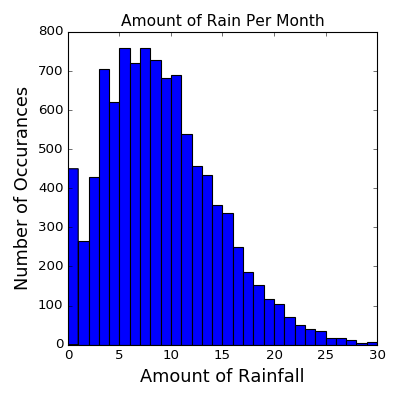
\includegraphics[width=0.40\textwidth]{Histogram.png}
\caption{Visual results of rainfall.\label{rain}}
\end{figure}

\subsection{Problem 3C}

This Problem asks to find the average amount of rain to fall in any given month. This is obtained by finding the sum of the variable "Swedish \textunderscore Fish" and dividing it by the number of months 

\subsection{Problem 3D}

This problem states that we want our approximations to problem three to be 95\% confident. To achieve this, The variable "Swedish \textunderscore Fish" is put into an array and organized such that it states the low edge 2.5\% of the data. A second line of code is created so that it takes away the top 2.5\% edge of the data. This gives us the 95 percentile of the data. The low edge of the data is 0 and the high edge is 21. I'm 95\% confident that the rainfall will be between 0 and 21 cm!


\end{document}
%%%%%%%%%%%%%%%%%%%%%%%%%%%%%%%%%%%%%%%%%%%%%%%%%%%%%%%%%%%%%%%%%%%%%%%%%%%%%%%%
